% --- SLIDE 4: PRUNING ---
\begin{frame}[fragile]{Pruning: Remove What Contributes Little}

    \begin{columns}[T]
        \begin{column}{0.53\textwidth}
            \begin{itemize}
                \small
                \item Trained networks are heavily over-parameterised: many weights barely affect the output.
                \item \textbf{Magnitude pruning:} remove the smallest weights, fine-tune the survivors to
                      recover accuracy, repeat. Han et al.\ (2015) cut AlexNet's weights $9\times$ and
                      VGG-16's $13\times$ with no loss of accuracy.
                \item \textbf{Unstructured} pruning zeroes individual weights: high compression, but a sparse
                      matrix runs no faster on standard kernels.
                \item \textbf{Structured} pruning removes whole channels, filters or layers: less compression,
                      but a smaller \emph{dense} model that is faster on any hardware.
            \end{itemize}
        \end{column}
        \begin{column}{0.45\textwidth}
            \centering
            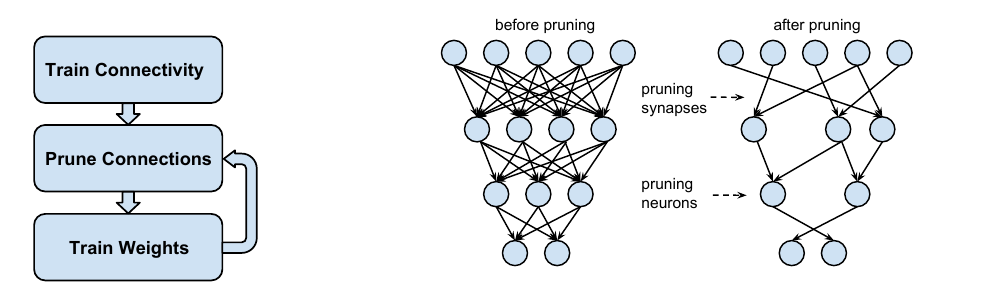
\includegraphics[width=\linewidth,height=0.4\textheight,keepaspectratio]{images/inference-optimisation/han_pruning_pipeline_synapses_neurons.png}\\[0.1em]
            {\scriptsize Han et al., \href{https://arxiv.org/abs/1506.02626}{arXiv:1506.02626}, Figures 2--3.}
            \vspace{0.3em}
    \begin{lstlisting}[language=Python, basicstyle=\ttfamily\scriptsize]
import torch.nn.utils.prune as prune
# zero the 50% smallest weights
prune.l1_unstructured(layer, "weight",
                      amount=0.5)
prune.remove(layer, "weight")
    \end{lstlisting}
        \end{column}
    \end{columns}

\end{frame}
